\section{RANSAC with Ellipse II (30)}
In this exercise, you are tasked to implement RANSAC algorithm for determining the shape of an ellipse in Python. The implementation must match your explanation in the report in order to receive full credits.

To test whether point $\mathbf{p}_i$ is an inlier, let the following inequality be the condition for inliers.
\begin{equation*}
    \left\|\sqrt{(\mathbf{p}_i-\mathbf{b})^\top\mathbf{Q}(\mathbf{p}_i-\mathbf{b})}-1\right\|\leq \varepsilon
\end{equation*}
where $\varepsilon$ is the tunable threshold.
\begin{enumerate}[a.)]
\item Based on the given template in Python, implement \textit{fit\textunderscore ellipse\textunderscore subset} that compute $\mathbf{Q}$ and $\mathbf{b}$ from a given set of points. (The number points is determined from 1.a). [8 pts] \\
\textbf{Answer}: \\
Plotting the ellipse from Question 1 yields:
\begin{figure}[H] % "H" ensures the image appears exactly here, can also use "h", "t", or "b" for positioning
    \centering
    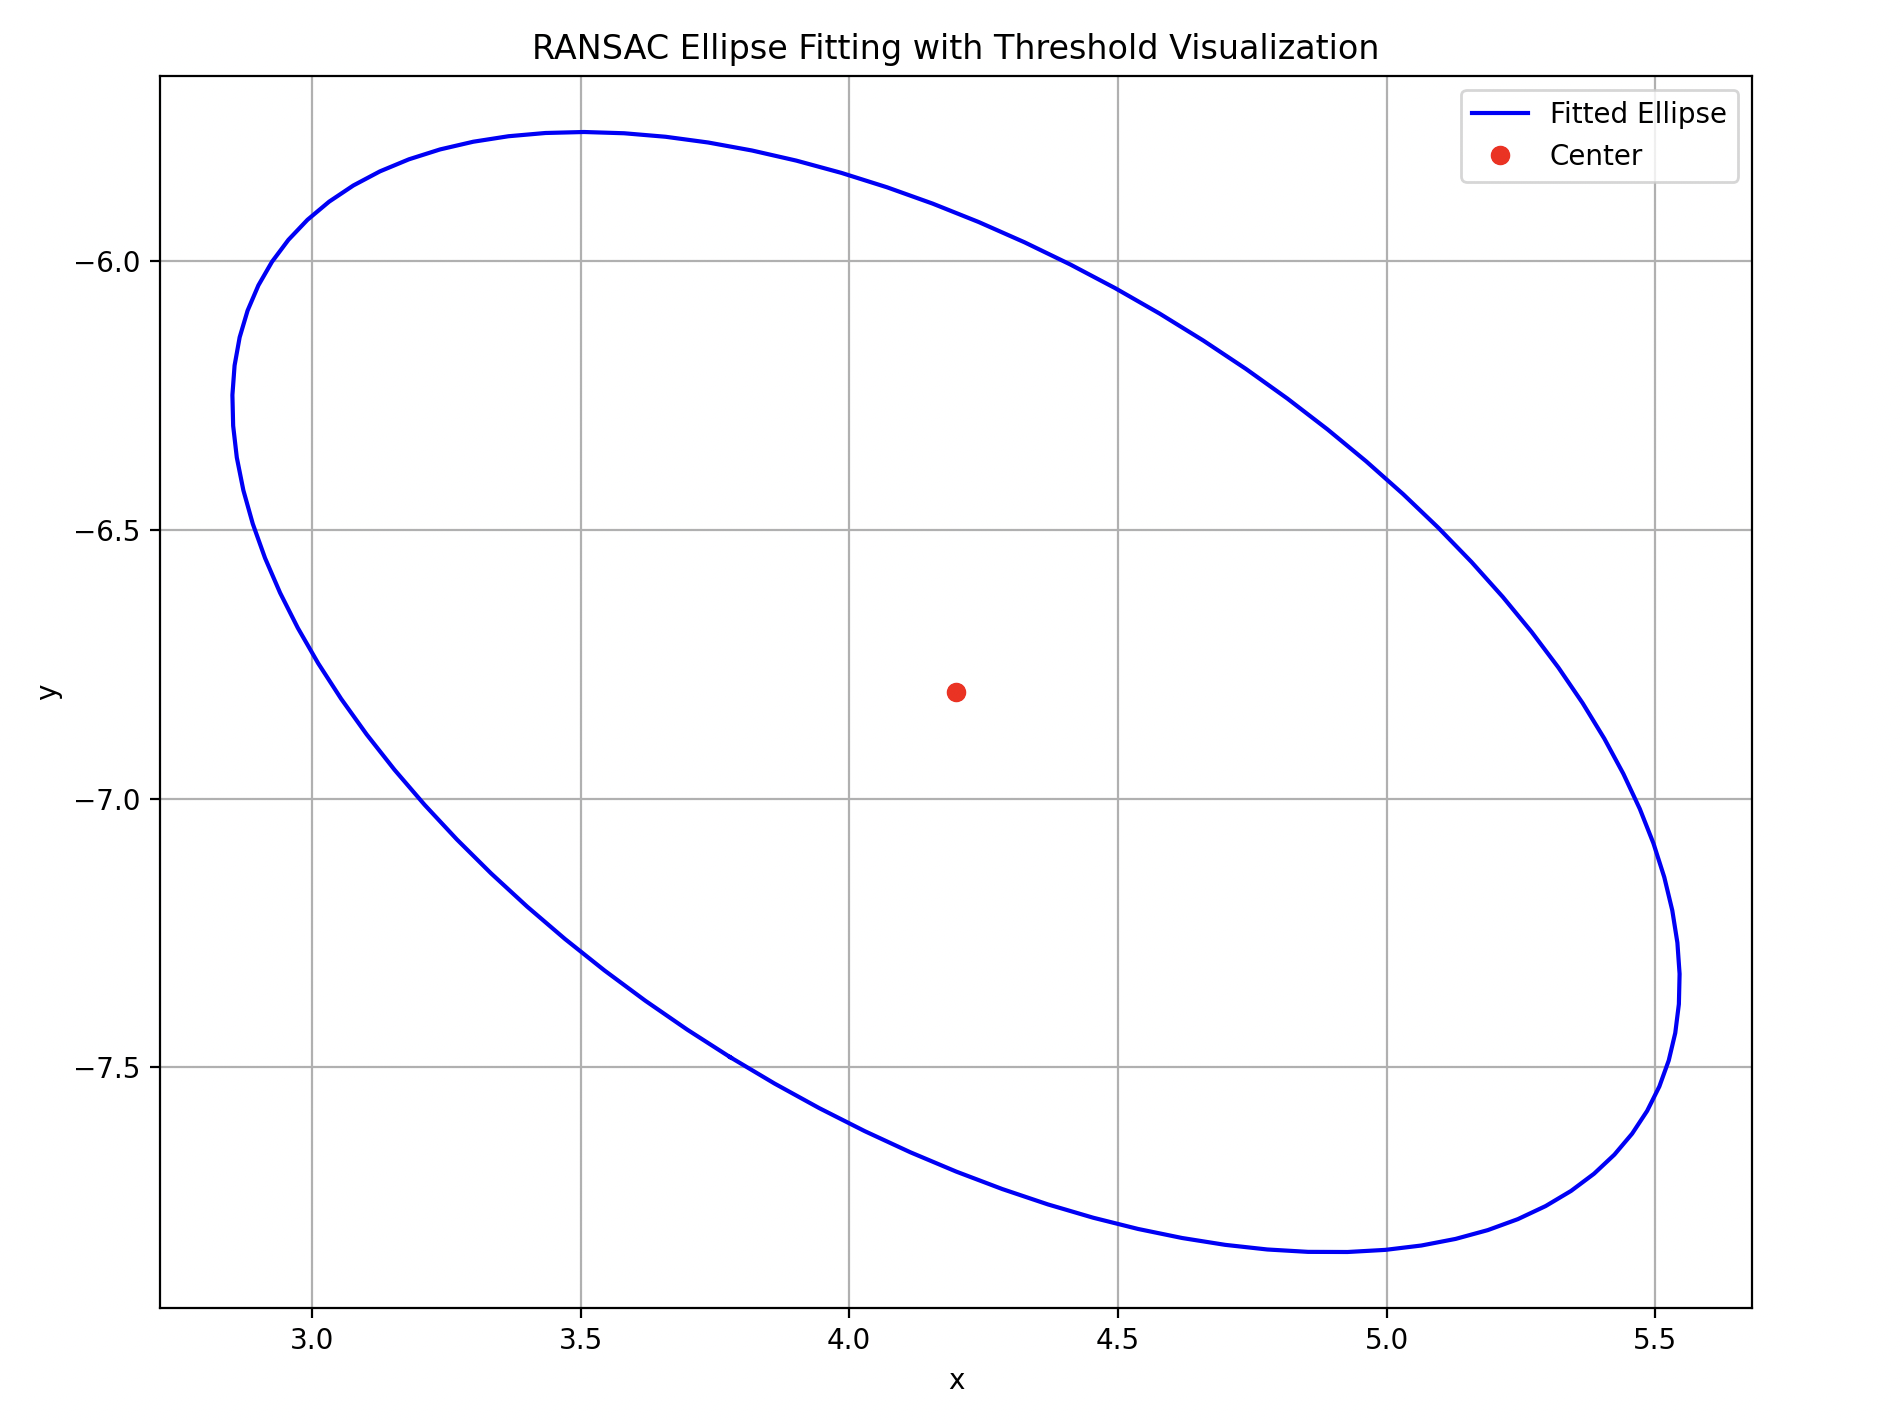
\includegraphics[width=0.5\textwidth]{/Users/kevinx/Desktop/MTE-544-assignments/assignment_2/assets/img/Figure_2.png} % adjust width as needed
    \caption{Question 1 Ellipse}
    \label{fig:your_label}
\end{figure}
\item Based on the given template in Python, implement \textit{ransac\textunderscore ellipse} that determined the best $\mathbf{Q}$, $\mathbf{b}$, and the corresponding inliers based on the given dataset, number of iterations, and threshold. You must explain your implementation step-by-step [12 pts]
 with the rationale in your report. \\
\textbf{Answer}: \\
 \textbf{Step 1}: \\
 Define three variables:
 1. Best set of inliers
 2. Best Q matrix 
 3. Best b vector 
 These will be updated according based on the error (distnace to inliers) of the fitted ellipse 
 
 \textbf{Step 2}: \\
 Create a \texttt{for} loop that runs the RANSAC algorithm for the number of iterations specified by \texttt{num\_iterations} and given a certain threshold. 
 
 Within the loop:
 \begin{itemize}
     \item Reset the \texttt{inliers} array to be empty.
     \item Select 5 random points from the input data.
     \item Use these 5 points to fit an ellipse, yielding \textbf{Q} and \textbf{b}.
     \item Determine the set of inliers corresponding to these 5 points based on the obtained \textbf{Q} and \textbf{b} matrices (detailed in further steps)
 \end{itemize}
 \textbf{Step 3}: \\
 Create an internal \texttt{for} loop to iterate through each point in the dataset. For each point, calculate its distance to the generated ellipse using the equation provided. If the calculated distance is less than the threshold, add the point to the \texttt{inliers} arary.
 
 \textbf{Step 4}: \\
 Make sure the ellipse is not too eccentric and the matrix \textbf{Q} is positive definite. If both of these conditions are not met, the \textbf{Q}, \textbf{b}, and inlier set are not used, even if the number of inliers found in the iteration was the highest so far.
 
 \textbf{Step 5}: \\
 If both of the conditions in \textbf{Step 4} are met, then compare the length of the current \texttt{inliers} array with that of the longest inliers array found so far. If the length of the current inliers array is longer, update \texttt{best\_inliers}, \texttt{best\_Q}, and \texttt{best\_b} accordingly. This concludes the algorithm.

 \textbf{Step 6}: \\
 Format the variables to be returned, then return them.

\item Based on the given template in Python, use different number of dataset, number of iterations, and threshold value. Comment on the effect of these parameters. [10 pts] \\
\\
\textbf{Answer}:
To evaluate the effects of each parameter, 3 different values of a single parameter were used, while leaving the other two parameters at their default values (dataset size = 500 points, number of iterations = 1000, threshold = 0.2). \textbf{Assumption}: The underlying nature of the data was randomly sample with noise from an ellipse. \\
\\
\textbf{Varying Dataset Size}: Experimenting with dataset sizes of 500, 1000, and 2000 \\
\begin{figure}[H] % "H" ensures the image appears exactly here, can also use "h", "t", or "b" for positioning
    \centering
    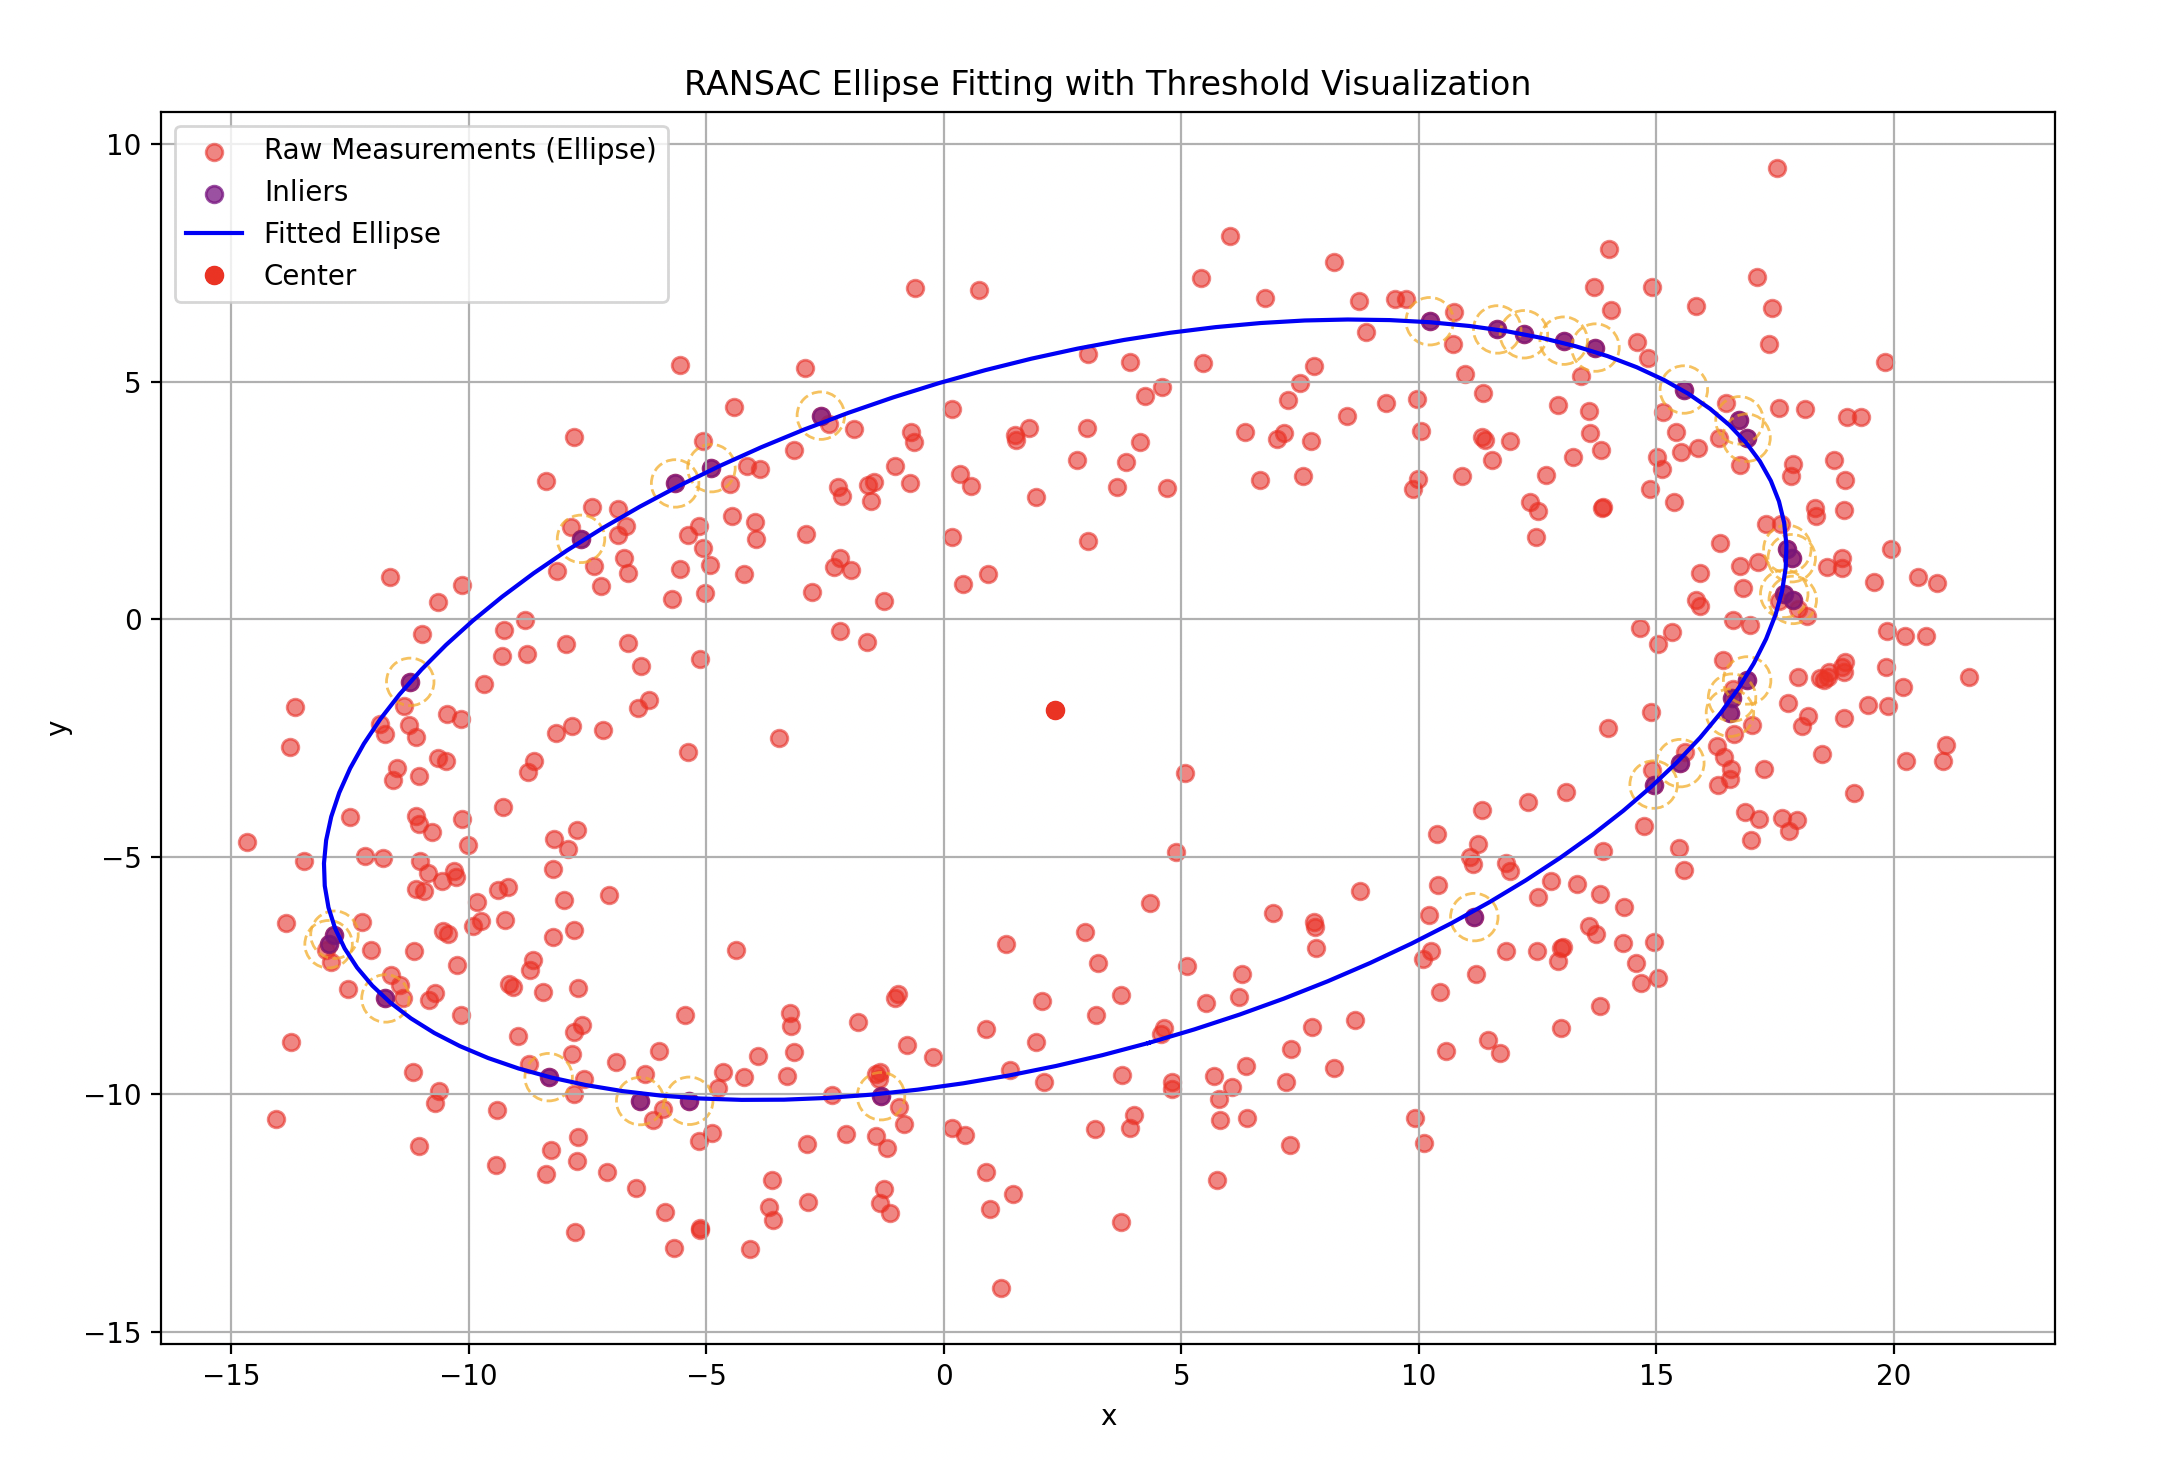
\includegraphics[width=0.5\textwidth]{/Users/kevinx/Desktop/MTE-544-assignments/assignment_2/assets/img/default.png} % adjust width as needed
    \caption{N = 500, Iterations = 1000, Threshold = 0.2}
    \label{fig:your_label}
\end{figure}
\begin{figure}[H] % "H" ensures the image appears exactly here, can also use "h", "t", or "b" for positioning
    \centering
    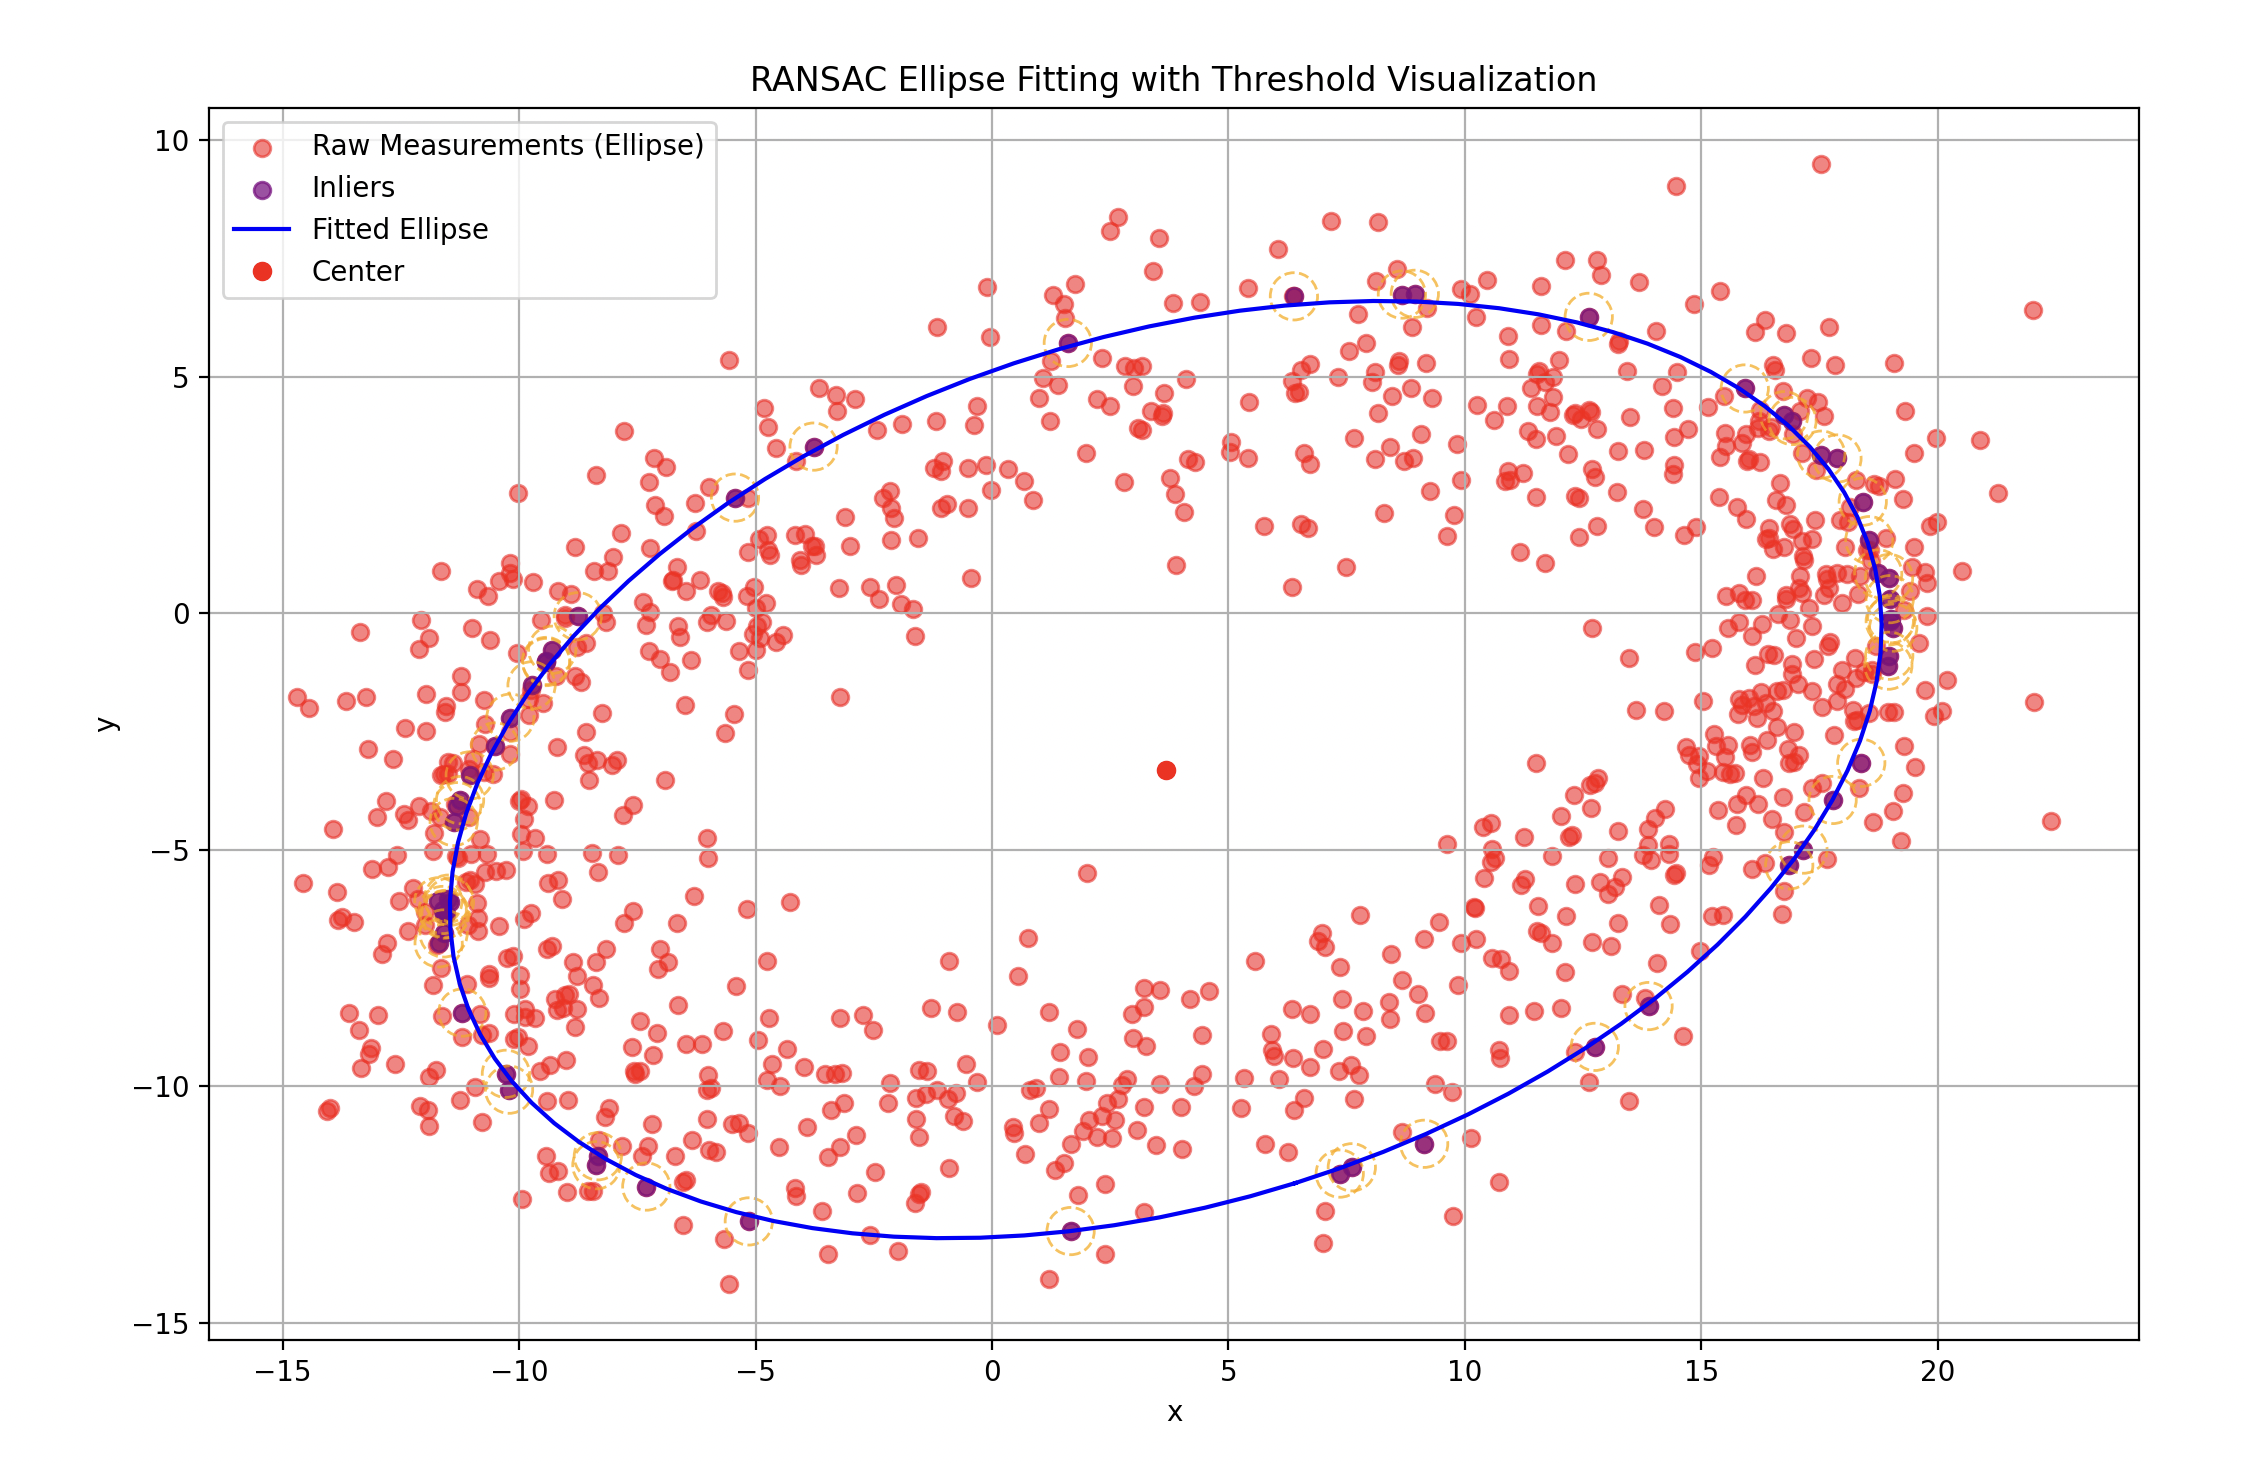
\includegraphics[width=0.5\textwidth]{/Users/kevinx/Desktop/MTE-544-assignments/assignment_2/assets/img/fig4.png} % adjust width as needed
    \caption{N = 1000, Iterations = 1000, Threshold = 0.2}
    \label{fig:your_label}
\end{figure}
\begin{figure}[H] % "H" ensures the image appears exactly here, can also use "h", "t", or "b" for positioning
    \centering
    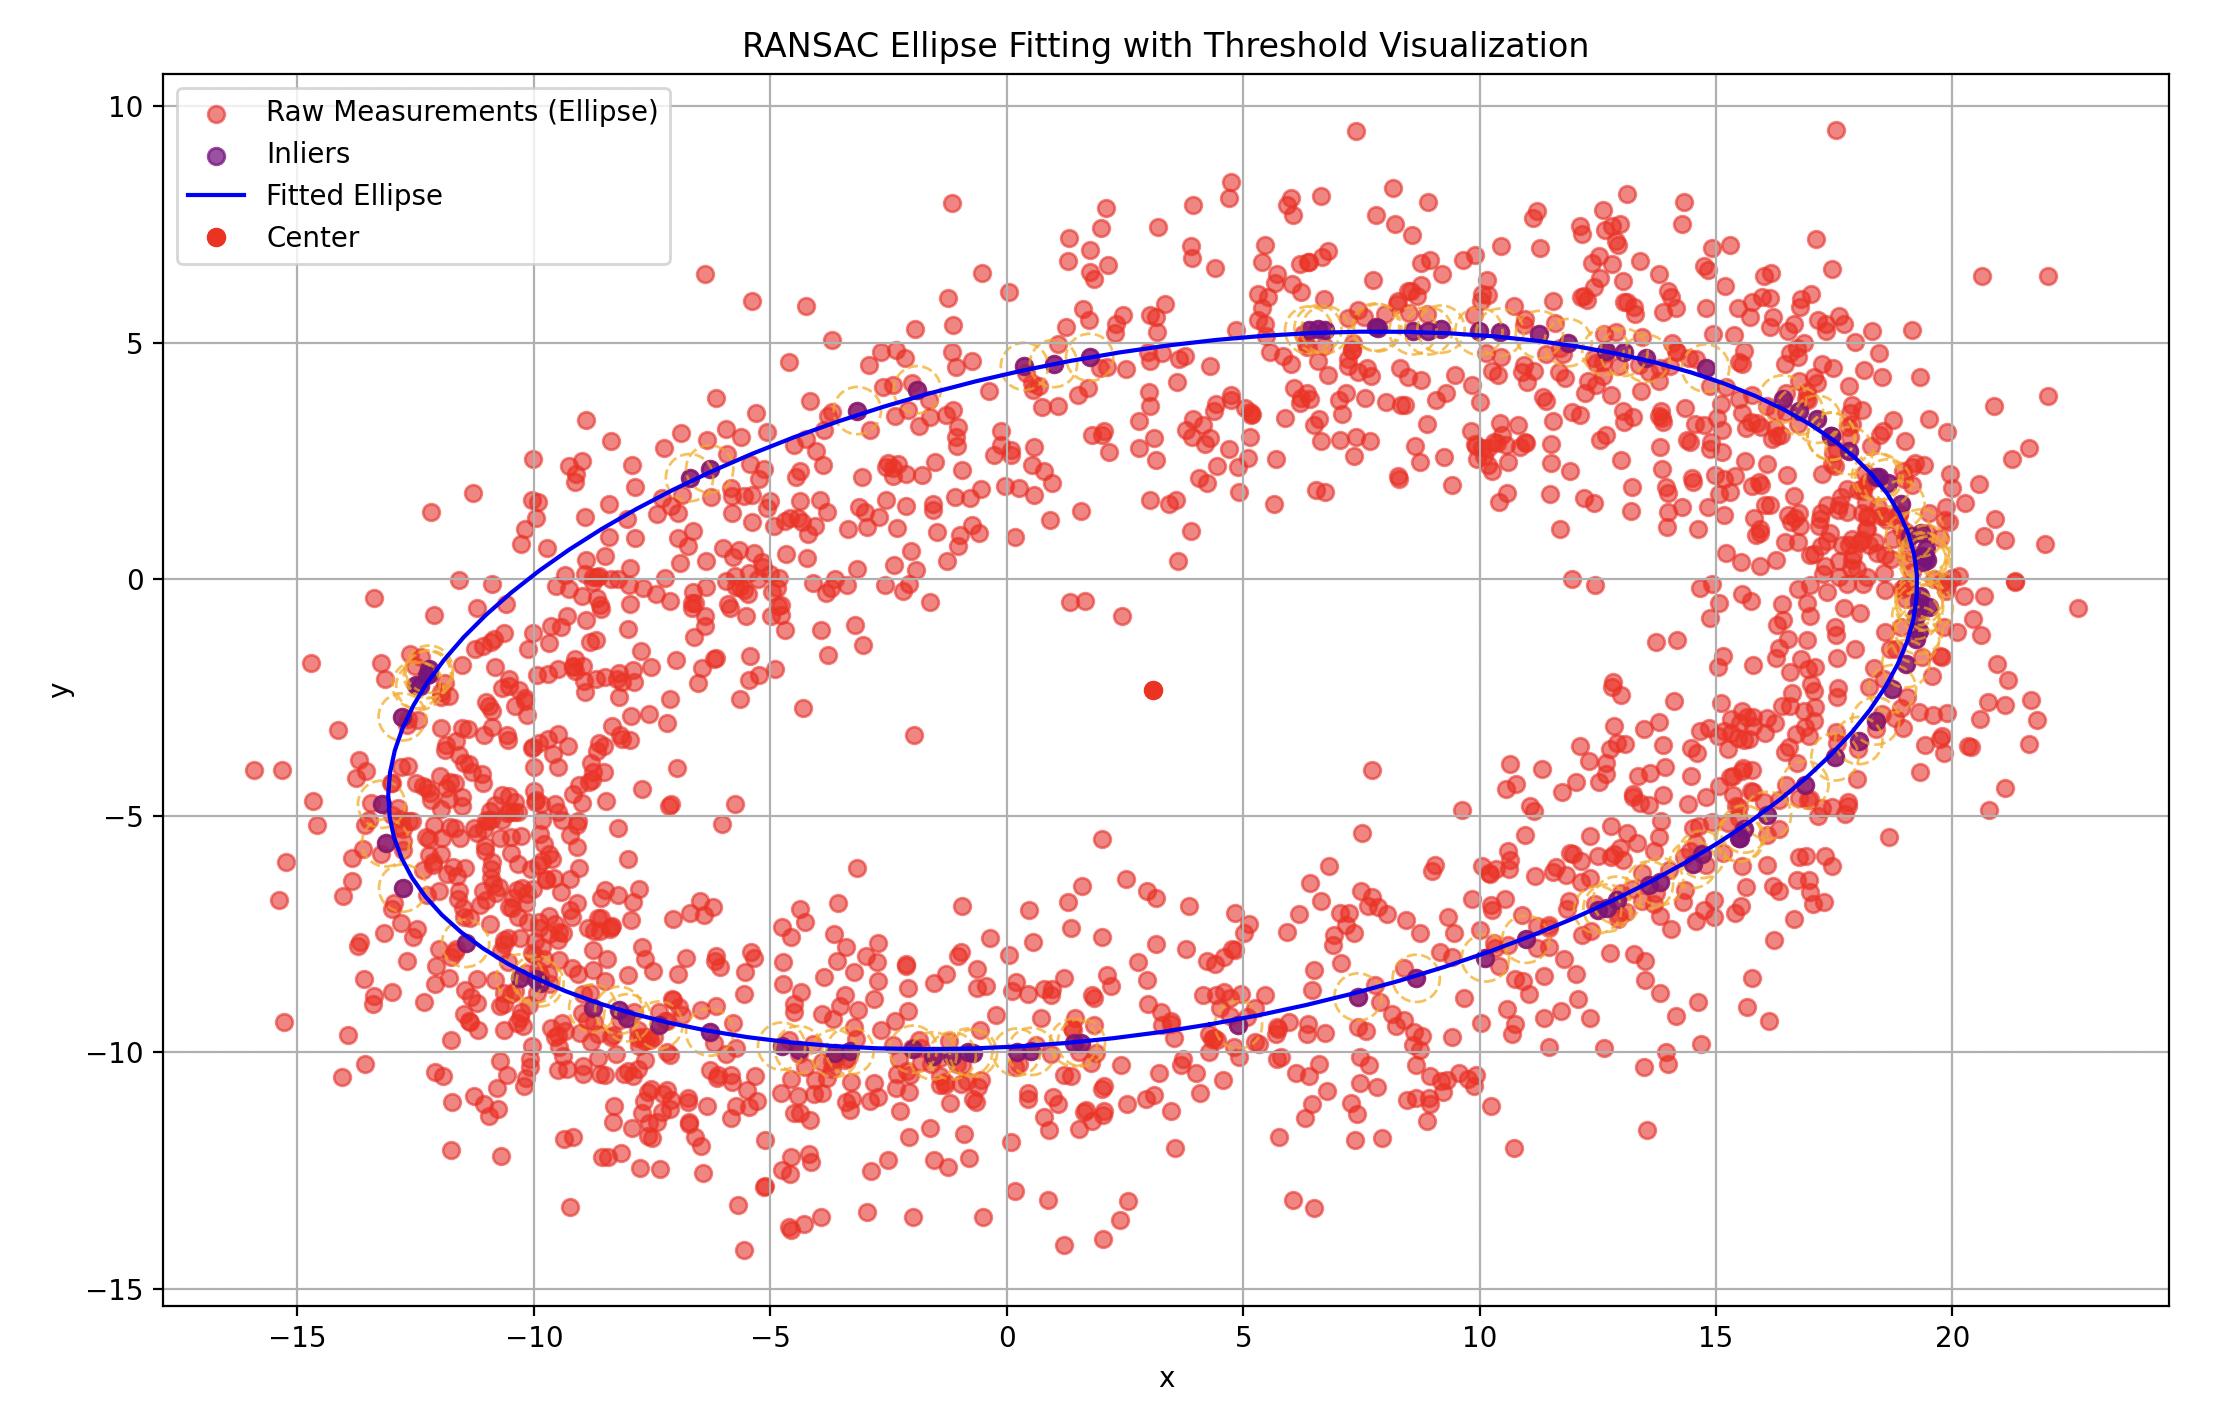
\includegraphics[width=0.5\textwidth]{/Users/kevinx/Desktop/MTE-544-assignments/assignment_2/assets/img/fig5.png} % adjust width as needed
    \caption{N = 2000, Iterations = 1000, Threshold = 0.2}
    \label{fig:your_label}
\end{figure}
It is evident that the higher the number of iterations, the more inliers there are, meaning that the parameters of the fitted ellipse more closely resemble the true parameters. \\

\textbf{Varying Number of Iterations}: Experimenting with iterations of 1000, 2000, 4000:
\begin{figure}[H] % "H" ensures the image appears exactly here, can also use "h", "t", or "b" for positioning
    \centering
    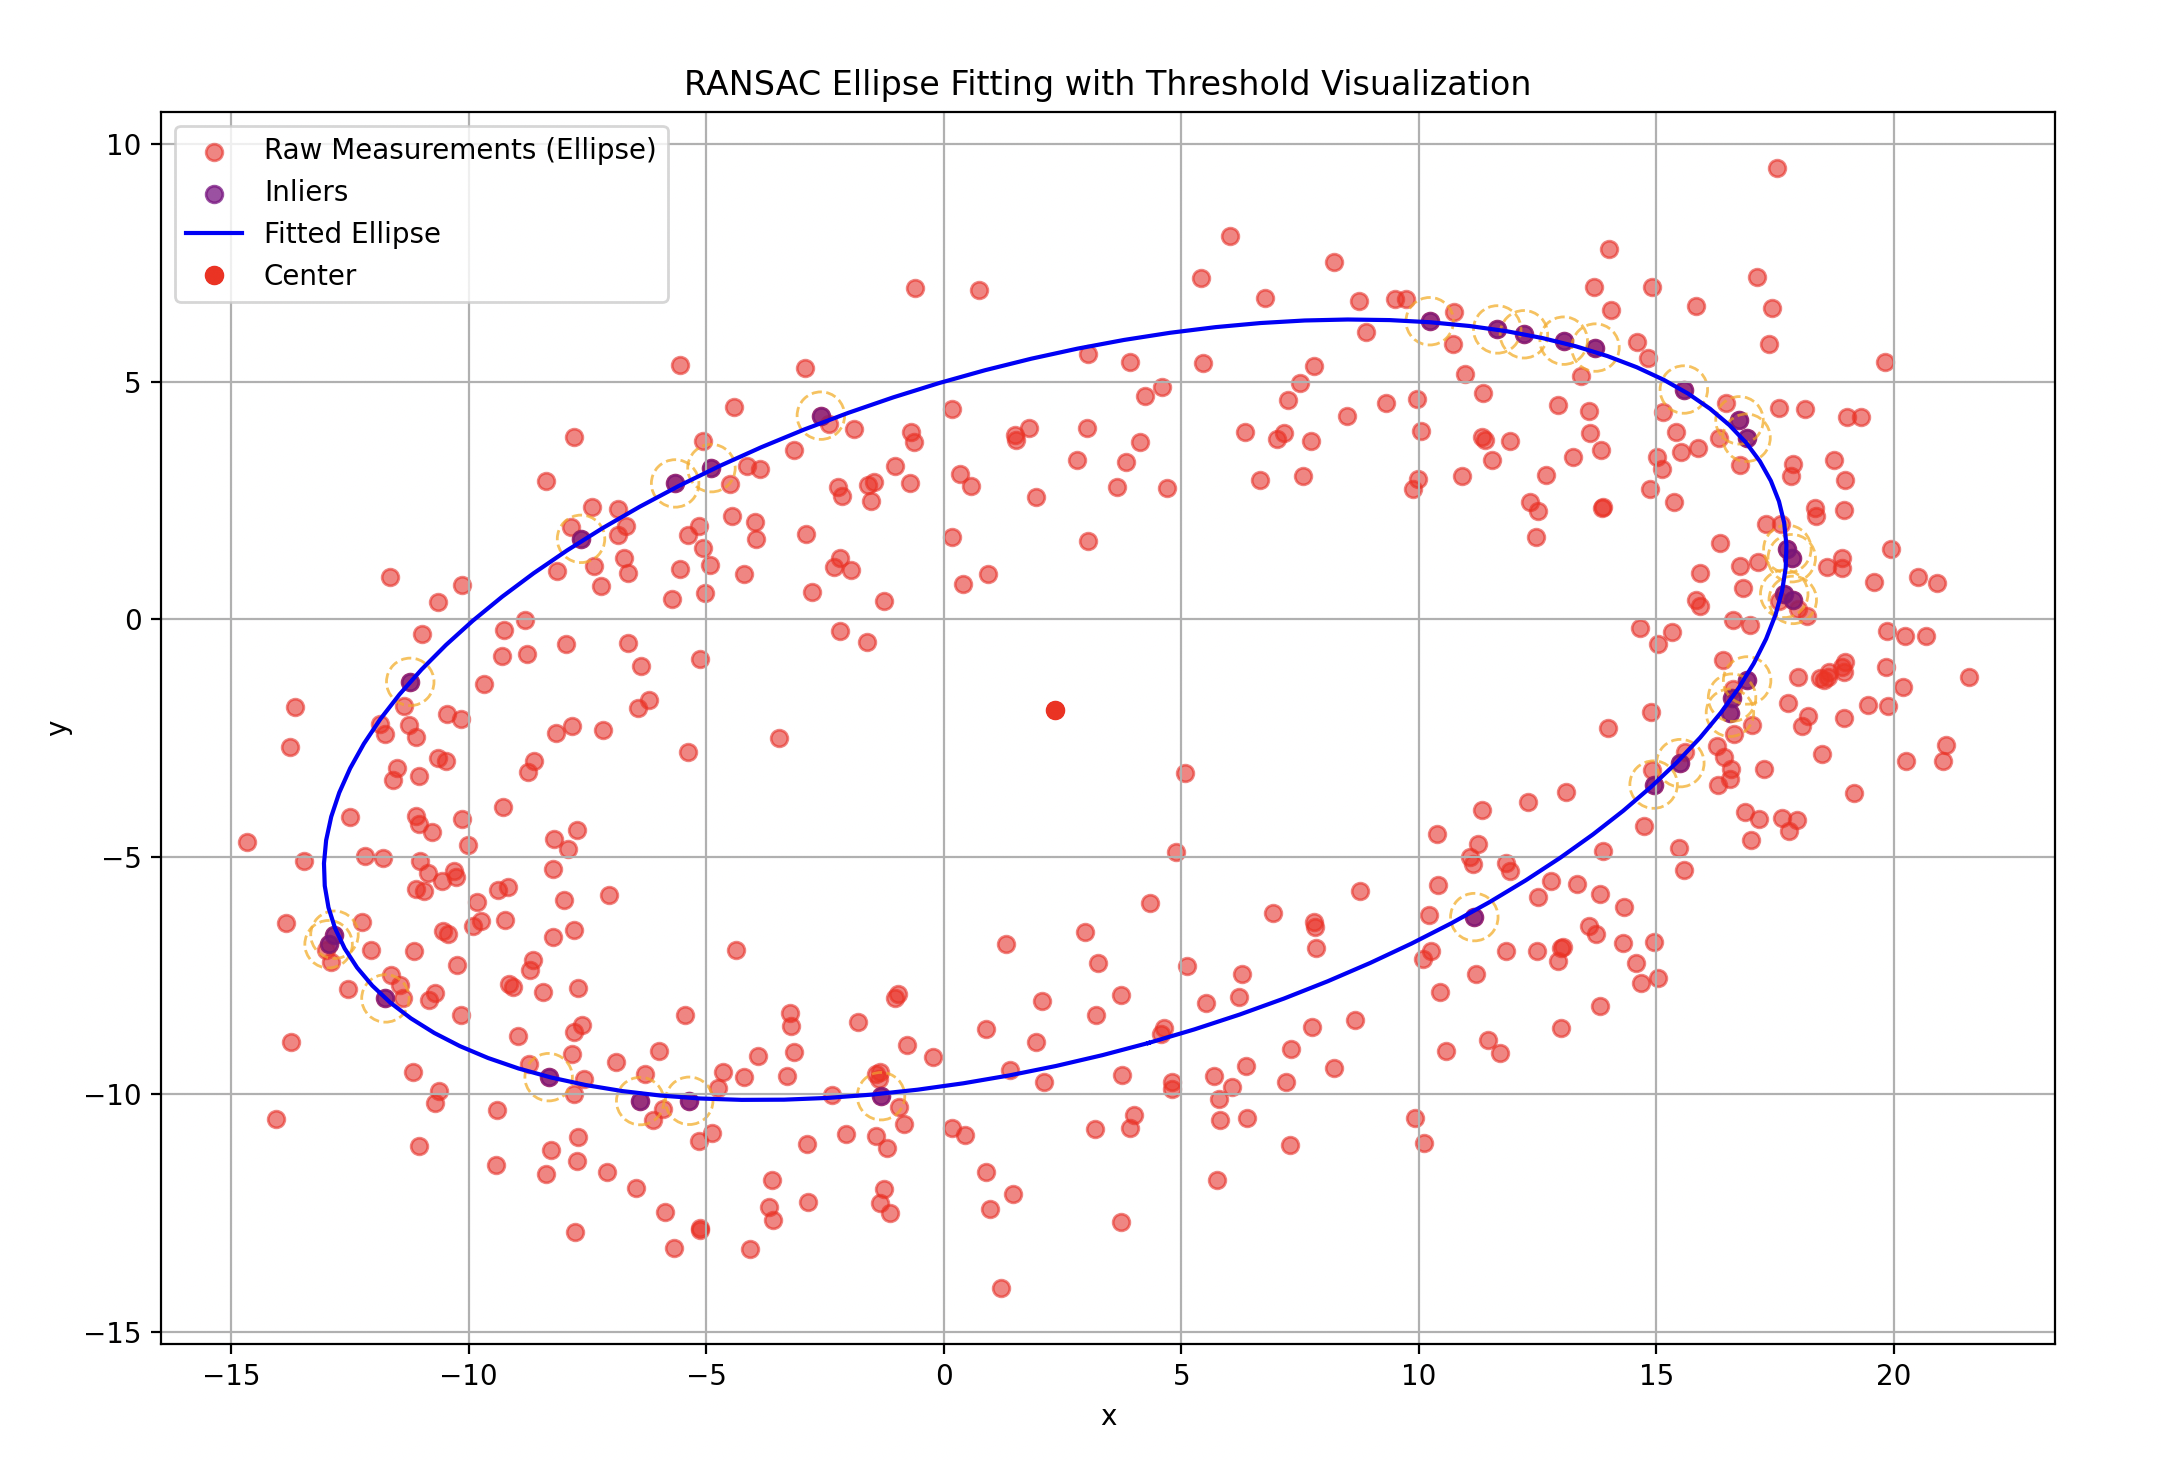
\includegraphics[width=0.5\textwidth]{/Users/kevinx/Desktop/MTE-544-assignments/assignment_2/assets/img/default.png} % adjust width as needed
    \caption{N = 500, Iterations = 1000, Threshold = 0.2}
    \label{fig:your_label}
\end{figure}
\begin{figure}[H] % "H" ensures the image appears exactly here, can also use "h", "t", or "b" for positioning
    \centering
    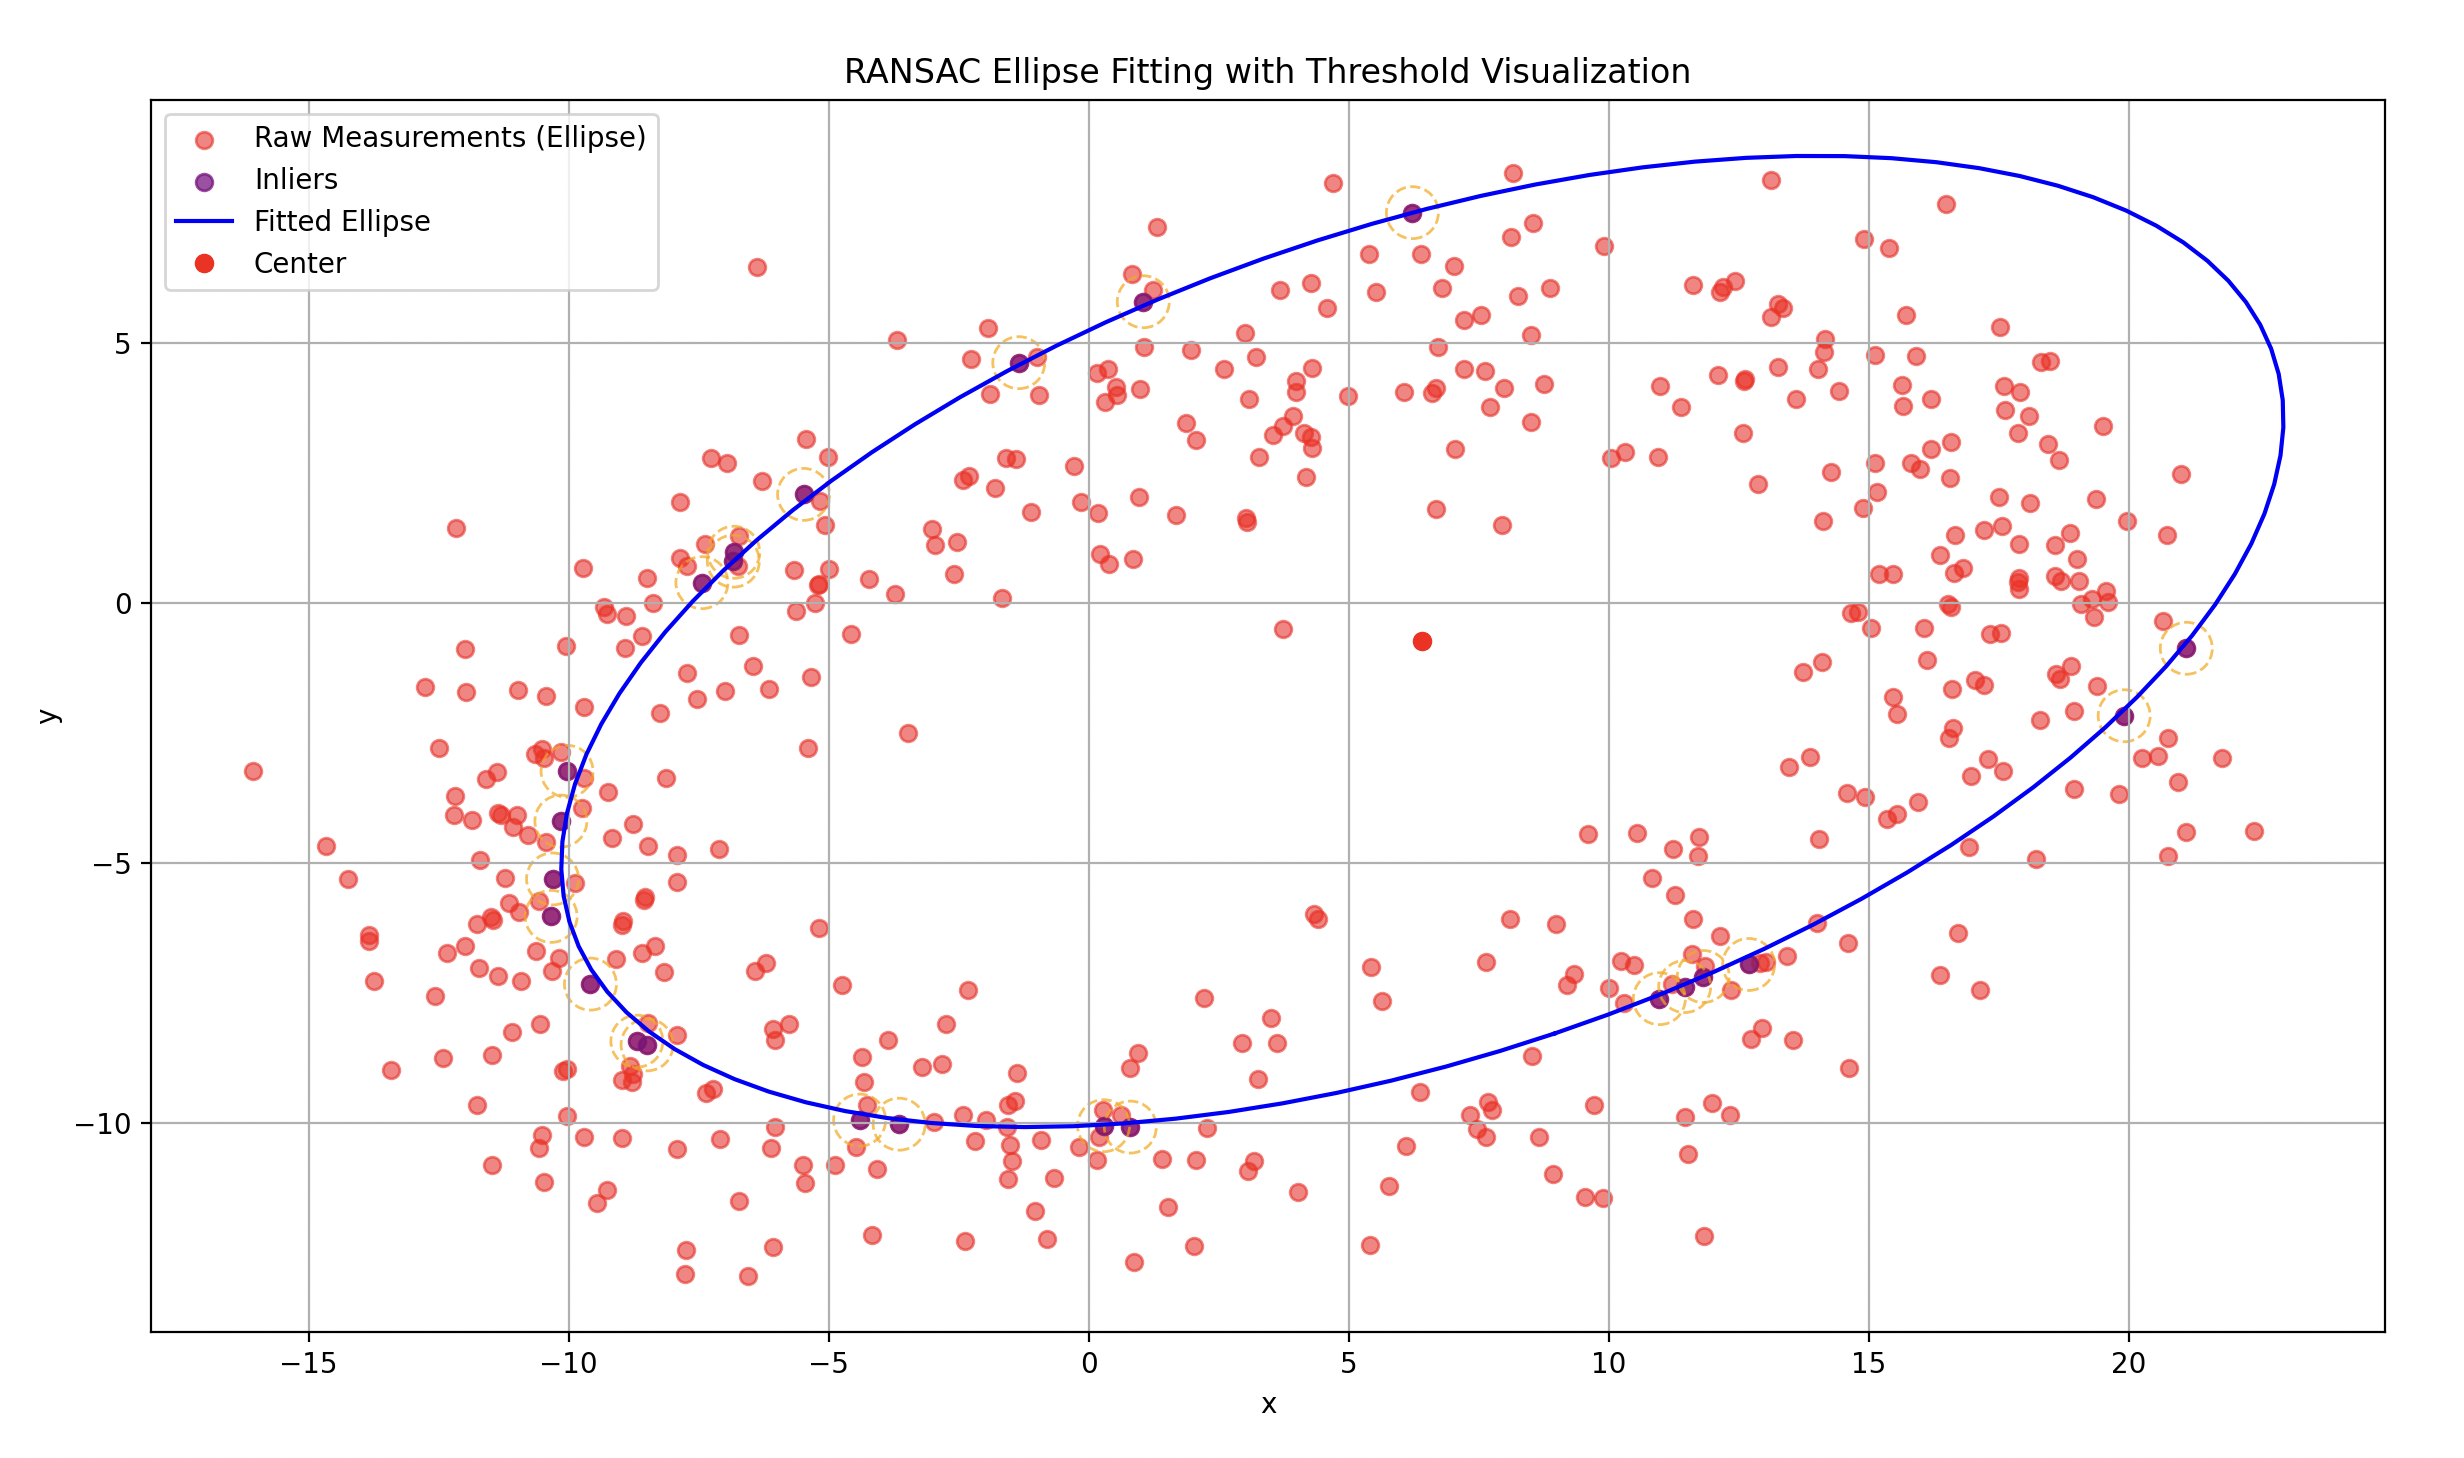
\includegraphics[width=0.5\textwidth]{/Users/kevinx/Desktop/MTE-544-assignments/assignment_2/assets/img/fig7.png} % adjust width as needed
    \caption{N = 500, Iterations = 100, Threshold = 0.2}
    \label{fig:your_label}
\end{figure}
\begin{figure}[H] % "H" ensures the image appears exactly here, can also use "h", "t", or "b" for positioning
    \centering
    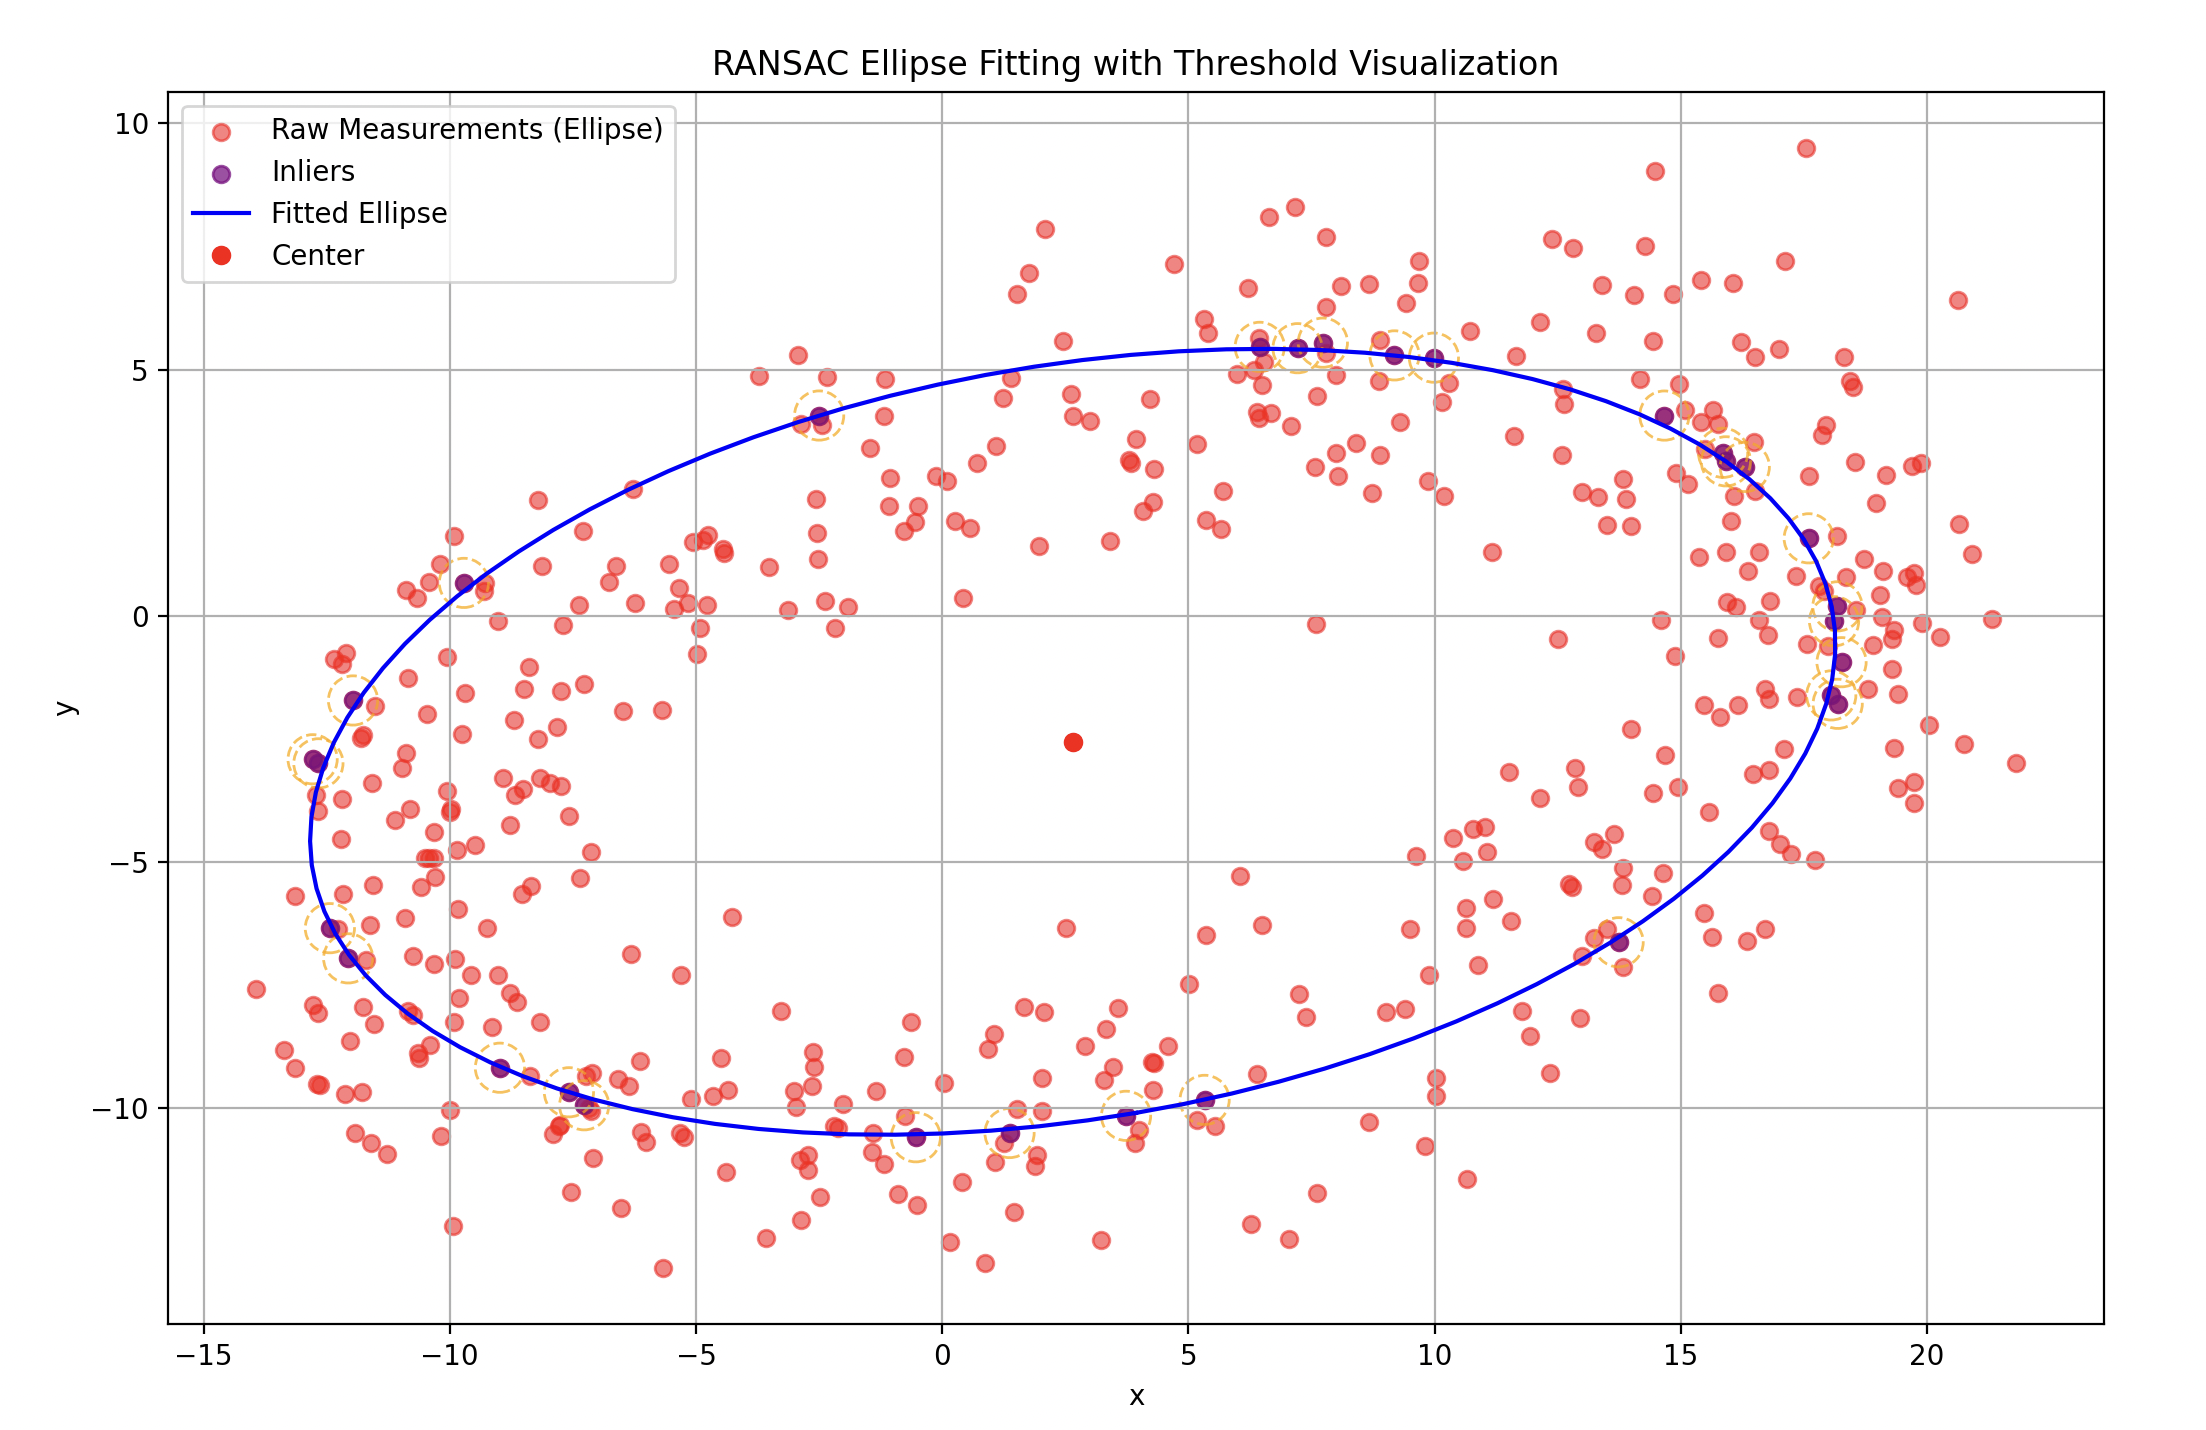
\includegraphics[width=0.5\textwidth]{/Users/kevinx/Desktop/MTE-544-assignments/assignment_2/assets/img/fig8.png} % adjust width as needed
    \caption{N = 500, Iterations = 3000, Threshold = 0.2}
    \label{fig:your_label}
\end{figure}
The results of modifying the number of iterations was somewhat expected, as the fitted ellipse had significant improvements with increasing iterations from 100 to 1000, but insignificant improvements with increasing iterations from 1000 to 3000.

\textbf{Varying Threshold}: Experimenting with thresholds of 0.2, 0.4, and 0.8:
\begin{figure}[H] % "H" ensures the image appears exactly here, can also use "h", "t", or "b" for positioning
    \centering
    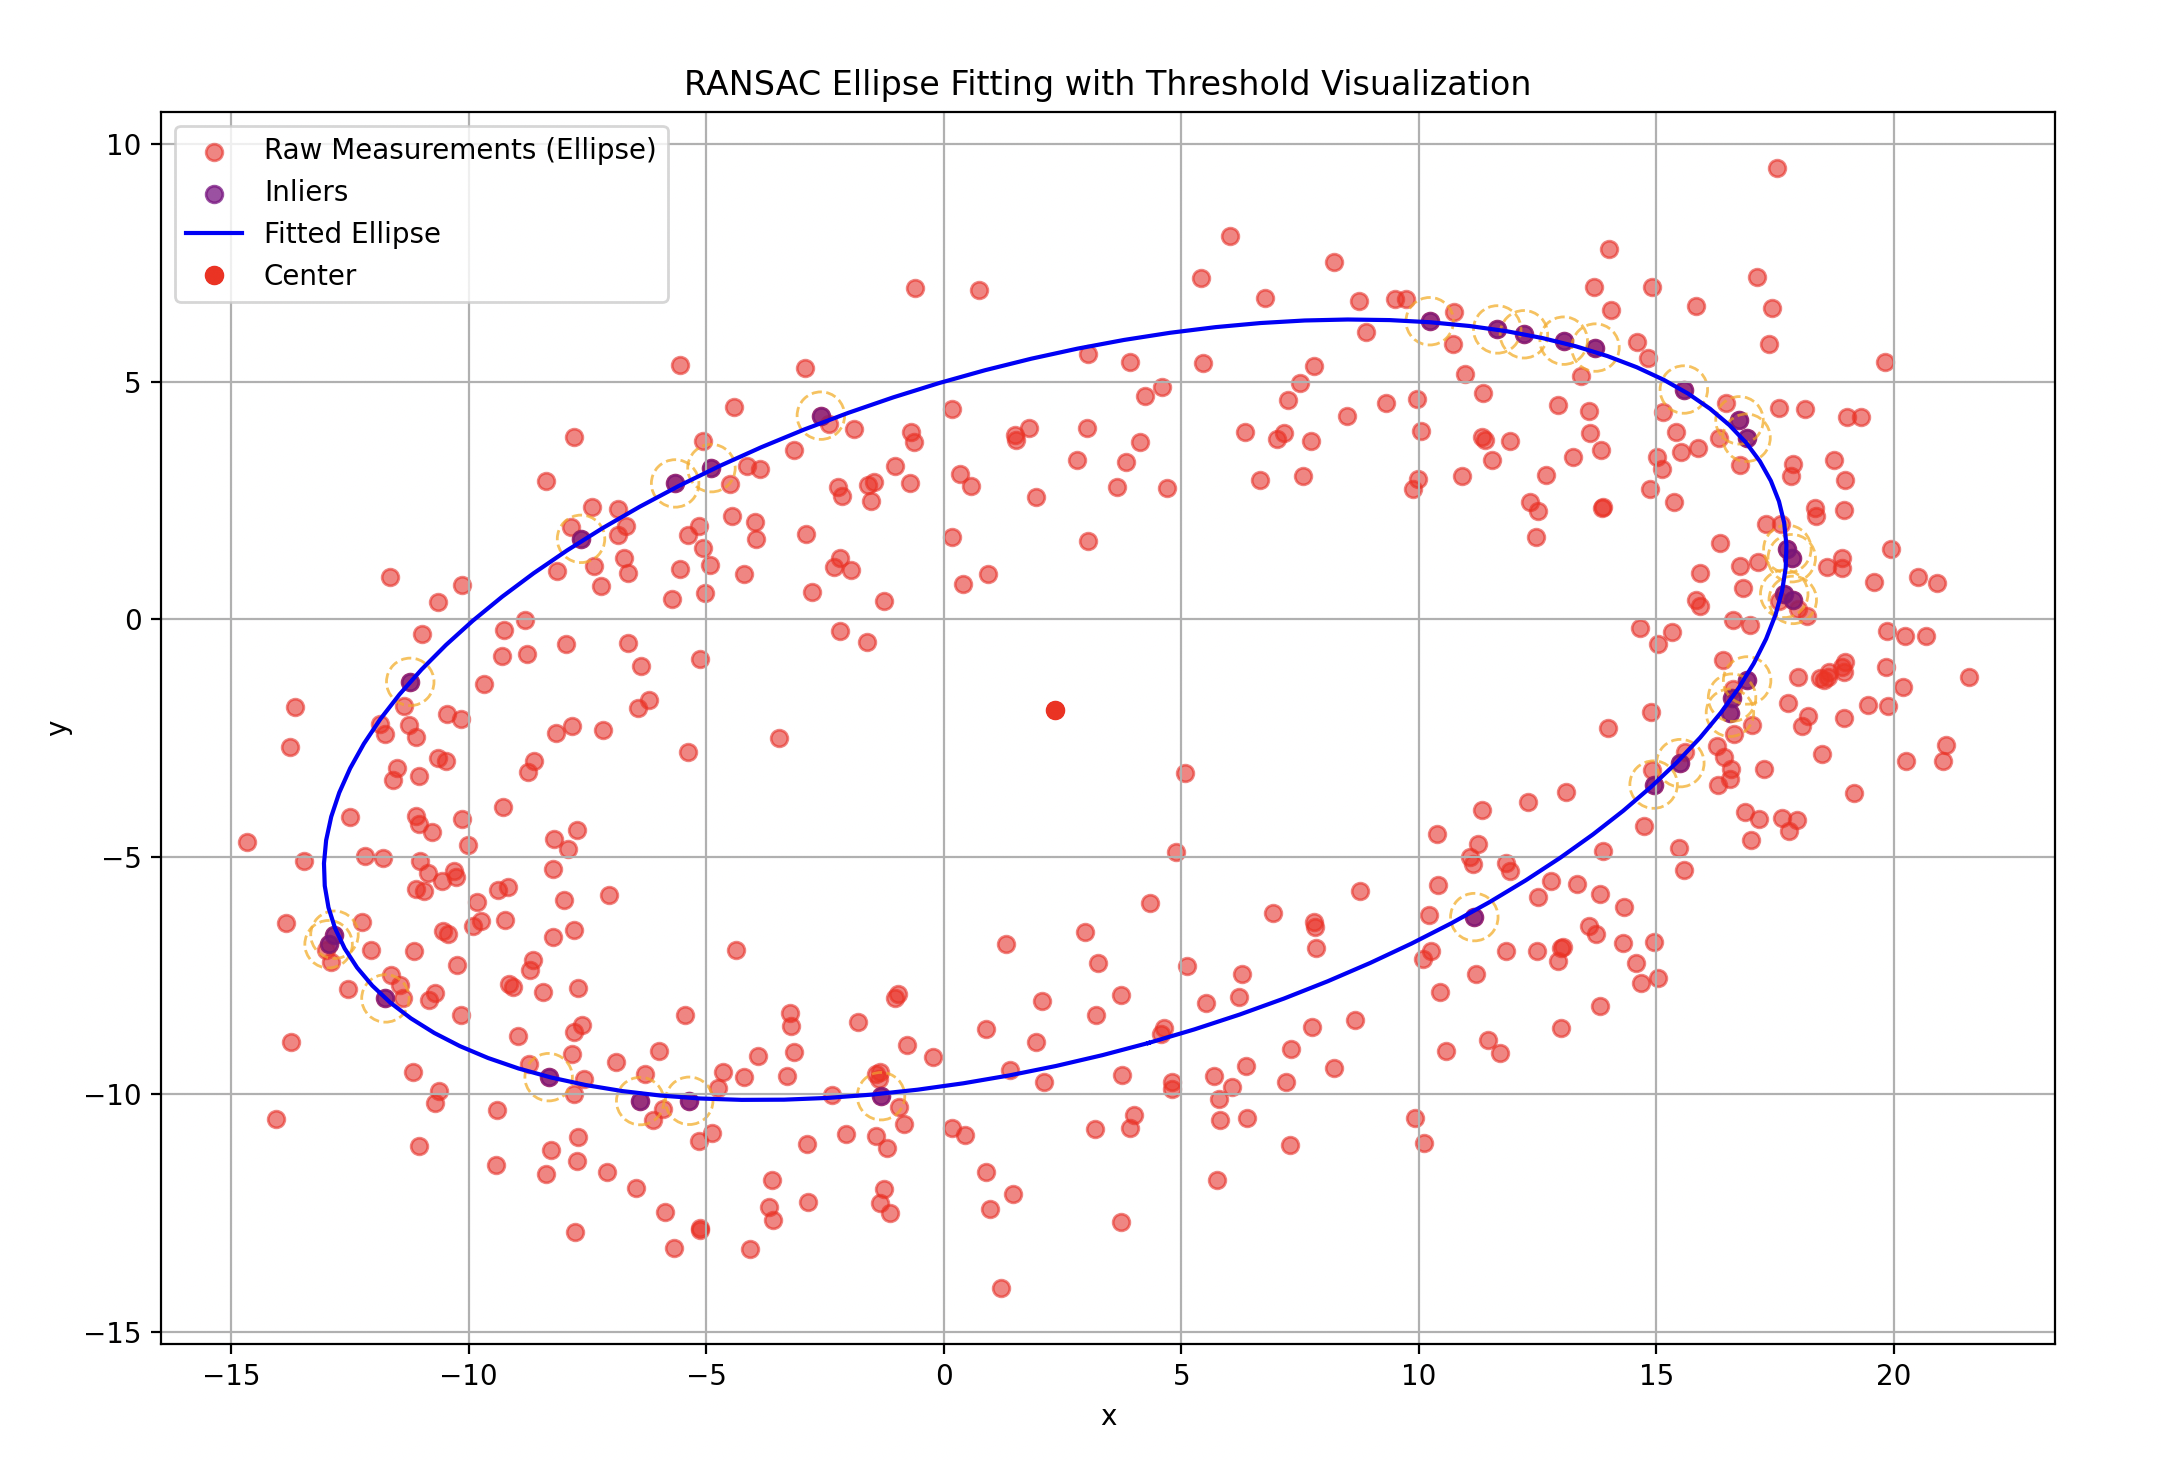
\includegraphics[width=0.5\textwidth]{/Users/kevinx/Desktop/MTE-544-assignments/assignment_2/assets/img/default.png} % adjust width as needed
    \caption{N = 500, Iterations = 1000, Threshold = 0.2}
    \label{fig:your_label}
\end{figure}
\begin{figure}[H] % "H" ensures the image appears exactly here, can also use "h", "t", or "b" for positioning
    \centering
    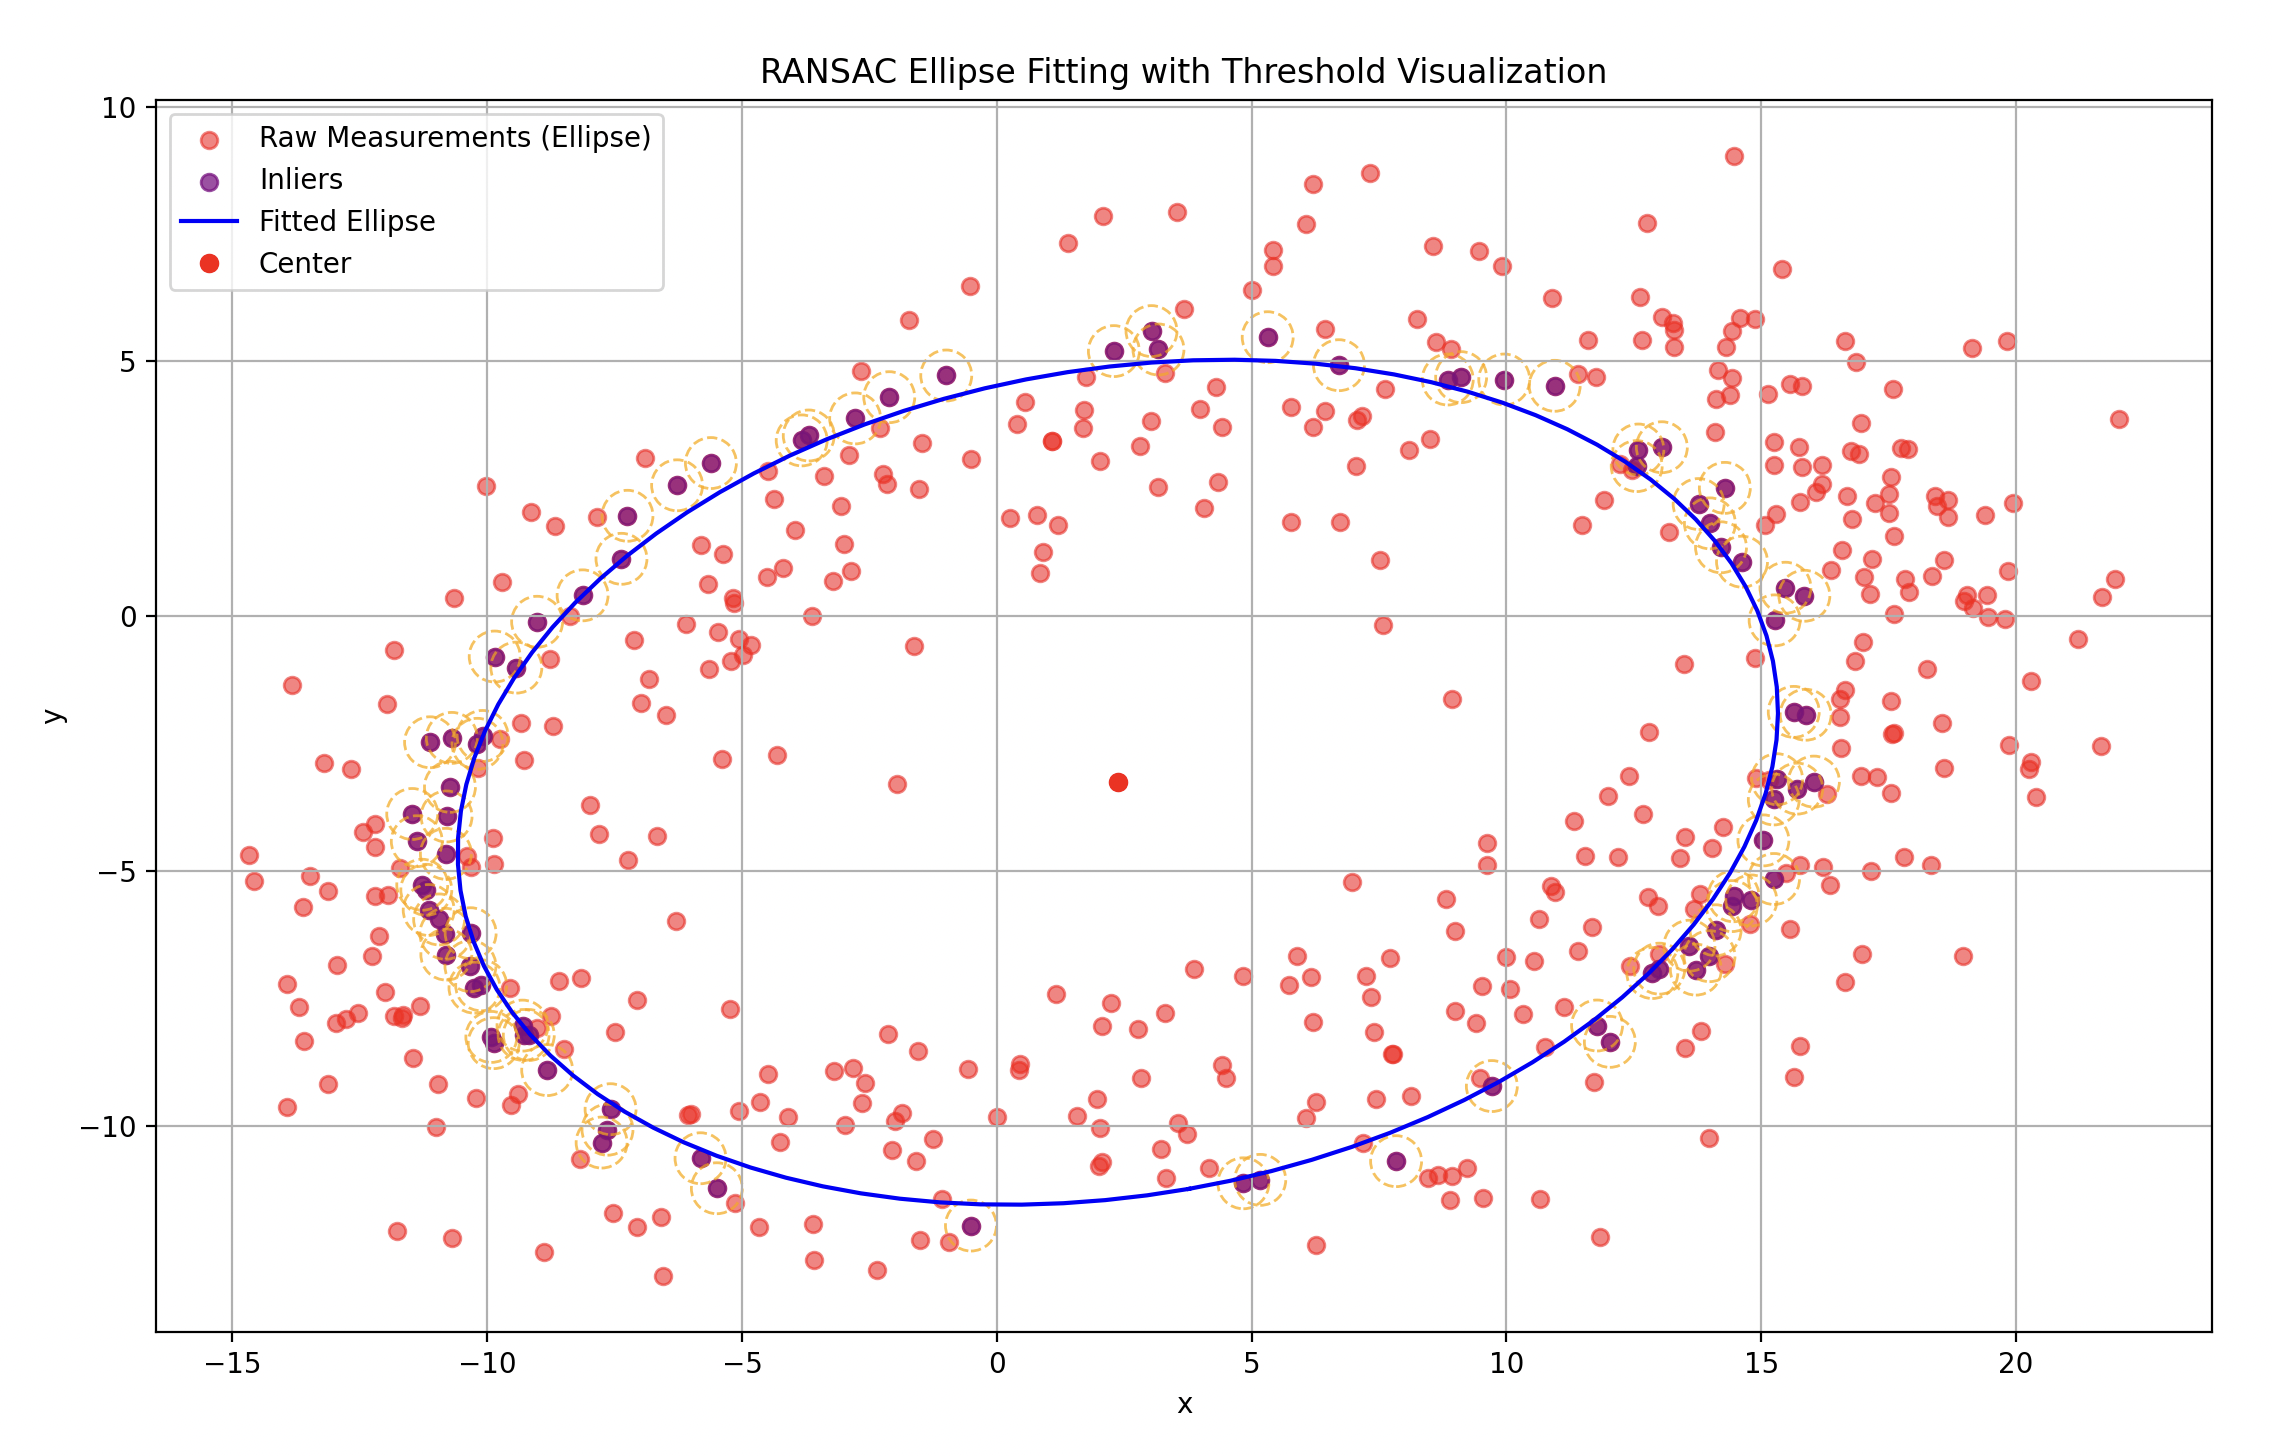
\includegraphics[width=0.5\textwidth]{/Users/kevinx/Desktop/MTE-544-assignments/assignment_2/assets/img/fig10.png} % adjust width as needed
    \caption{N = 500, Iterations = 1000, Threshold = 0.4}
    \label{fig:your_label}
\end{figure}
\begin{figure}[H] % "H" ensures the image appears exactly here, can also use "h", "t", or "b" for positioning
    \centering
    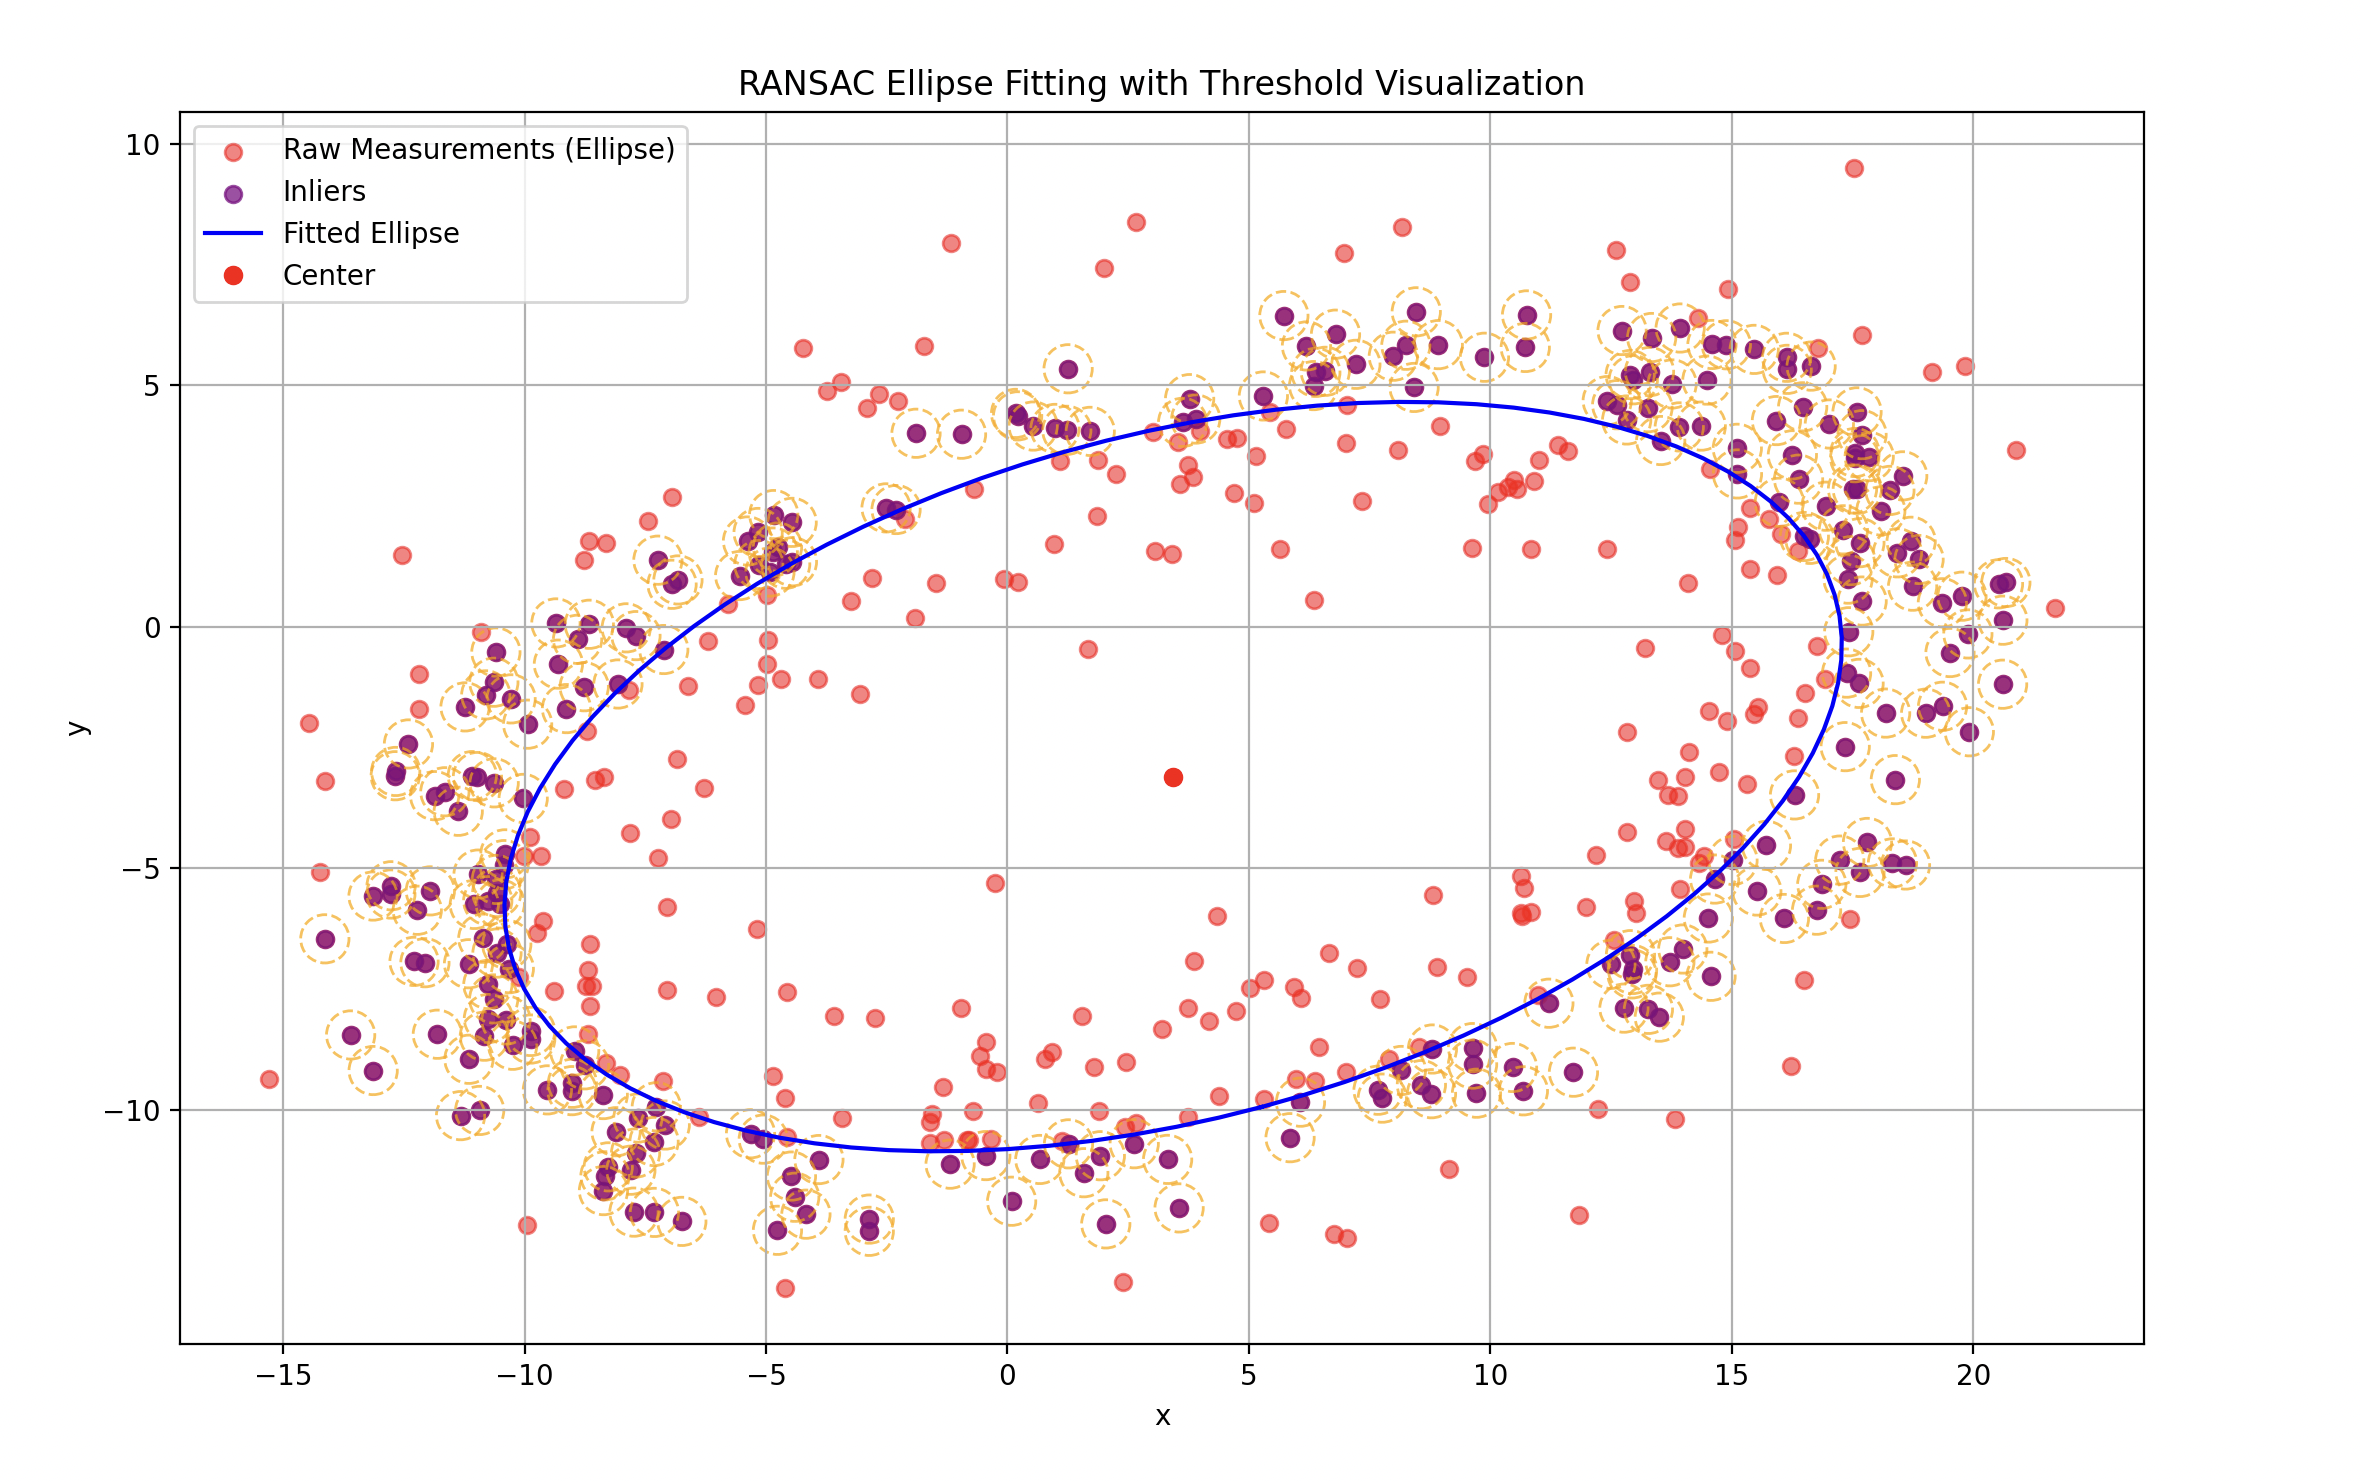
\includegraphics[width=0.5\textwidth]{/Users/kevinx/Desktop/MTE-544-assignments/assignment_2/assets/img/fig11.png} % adjust width as needed
    \caption{N = 500, Iterations = 2000, Threshold = 0.8}
    \label{fig:your_label}
\end{figure}
The results of modifying the threshold was as expected, as increasing the threshold is expected to increase the number of inliers which satisfy the condition.

\end{enumerate}